\documentclass{../../../oss-apphys-exam}
\usepackage{bm}
\usepackage{enumitem}

\usetikzlibrary{decorations.pathmorphing,patterns}

\renewcommand{\arraystretch}{1.5}
\usepackage{circuitikz} % to draw circuits!
\ctikzset{bipoles/length=.8cm}

\raggedcolumns

\runningheader{
  \fontfamily{phv}\small
  \textcolor{gray}{AP PHYSICS C: ELECTRICITY AND MAGNETISM $\blacksquare$}
  \textbf{FREE-RESPONSE QUESTIONS}}{}{}


\begin{document}

\gentitle{10}{FARADAY'S LAW, PART 2}

  

\begin{questions}
  
  % TAKEN FROM THE 2014 AP PHYSICS EXAM QUESTION E&M.2
  \uplevel{\
    \centering
    \begin{tikzpicture}[scale=1.1]
      \draw[axes] (-1,0)--(6,0) node[right]{$x$};
      \draw (0,.1)--(0,-.1) node[below]{$O$};
      \draw (1,.1)--(1,-.1) node[below]{$L$};
      \foreach \x in {2,...,5} \draw (\x,.1)--(\x,-.1) node[below]{\x$L$};
      \foreach \x in {1,3}\draw[dashed] (\x,0)--(\x,2.35);
      \foreach \x in {-.7,3.4} \draw[thick] (\x,1.1) rectangle +(1,.3);
      \draw[vectors] (.4,1.25)--+(.8,0) node[midway,above=-1]{$v_0$};
      \draw[vectors] (4.5,1.25)--+(.8,0) node[midway,above=-1]{$v_f$};
      \foreach \x in {1.2,1.6,...,3} {
        \foreach \y in {.3,.9,...,2.3} \node at (\x,\y) {$\bm\times$};
      }
      \draw[|<->|] (-.7,.85)--+(1,0) node[midway,fill=white]{$L$};
      \draw[->|] (-.85,1.8)--+(-0,-.4);
      \draw[->|] (-.85,.7)--+(-0,.4);
      \node[left] at (-.9,1.25) {$L/4$};
    \end{tikzpicture}
  }
  \question The rectangular loop of wire shown on the left in the figure above
  has mass $M$, length $L$, width $L/4$, and resistance $R$. It is initially
  moving to the right at constant speed $v_0$ , with no net force acting on
  it. At time $t=0$ the loop enters a region of length $2L$ that contains a
  uniform magnetic field of magnitude $B$ directed into the page. The loop
  emerges from the field at time $t_f$ with final speed $v_f$. Express all
  algebraic answers to the following in terms of $M$, $L$, $R$, $B$, $v_0$,
  and fundamental constants, as appropriate.
  \begin{parts}
    \part Let $x$ represent the position of the right end of the loop. Place a
    check mark in the appropriate box in each column in the table below to
    indicate whether the speed of the loop increases, decreases, or stays the
    same as the loop moves to the right.
    \uplevel{
      \centering
      \begin{tabular}{|c|c|c|c|c|}
        \hline
        & \multicolumn{4}{c|}{Position of Right End of Loop} \\ \hline
        Speed of Loop & $L<x<2L$ & $2L<x<3L$ & $3L<x<4L$ & $4L<x<5L$ \\
        \hline
        Increases & & & & \\
        \hline
        Dereases & & & & \\
        \hline
        Stays the Same & & & & \\
        \hline
      \end{tabular}
    }

    \part\textbf{Derive} an expression for the magnitude of the current induced
    in the loop as its right edge enters the field.
    \vspace{\stretch1}
    
    \part\textbf{Indicate} the direction of the induced current determined in
    part \textbf{B}.

    \vspace{.1in}
    \underline{\hspace{.3in}} Clockwise\hspace{.5in}
    \underline{\hspace{.3in}} Counterclockwise
    
    \vspace{.15in}\textbf{Justify} your answer.
    \vspace{\stretch1}
    \newpage
    
    \part\textbf{Write}, but do not solve, a differential equation for the speed
    $v$ as a function of time as the loop enters the field.
    \vspace{\stretch1}
    
    \part\textbf{Indicate} the direction of the acceleration of the loop just
    before its left edge leaves the field?

    \vspace{.1in}
    \underline{\hspace{.3in}} Left\hspace{1in}
    \underline{\hspace{.3in}} Right\hspace{1in}
    \underline{\hspace{.3in}} Up\hspace{1in}
    \underline{\hspace{.3in}} Down
  
    \vspace{.1in}\textbf{Justify} your answer.
    \vspace{\stretch4}
  \end{parts}
  \newpage

  \uplevel{
    \centering
    \begin{tikzpicture}[scale=1.2]
      \foreach \x in {0,...,3}{
        \foreach \y in {0,...,4} \node at (\x,\y){\color{gray}$\times$};
      }
      \draw[thick,fill=lightgray] (.5,2.25) rectangle (2.5,2.5)
      node[above=1,midway]{$M,L$};
      \draw[thick](.5,.5)--(.5,3.7) node[pos=0,left]{$B$}
      to[R,l=$R$](2.5,3.7)--(2.5,.5);
      \fill (1.5,1.5) circle (.06) node[right]{D};
      \fill (1.5,3.2) circle (.06) node[right]{C};
      \draw[vectors] (4.5,3)--(4.5,2) node[below]{Vertically down};
    \end{tikzpicture}
  }
  \question A conducting bar of mass $M$, length $L$, and negligible resistance
  is connected to two long vertical conducting rails of negligible resistance.
  The two rails are connected by a resistor of resistance $R$ at the top. The
  entire apparatus is located in a magnetic field of magnitude $B$ directed
  into the page, as shown in the figure above. The bar is released from rest
  and slides without friction down the rails.
  \begin{parts}
    \part\textbf{Indicate} the direction of the current in the resistor.
    
    \vspace{.1in}
    \underline{\hspace{.3in}} Left\hspace{.5in}
    \underline{\hspace{.3in}} Right

    \vspace{.15in}\textbf{Justify} your answer.
    \vspace{\stretch1}
    
    \part\textbf{Indicate} whether the magnitude of the net magnetic field
    above the bar at point C greater than, less than, or equal to the magnitude
    of the net magnetic field before the bar is released.
    
    \vspace{.1in}
    \underline{\hspace{.3in}}Greater than\hspace{.5in}
    \underline{\hspace{.3in}}Less than\hspace{.5in}
    \underline{\hspace{.3in}}Equal to

    \vspace{.15in}\textbf{Justify} your answer.
    \vspace{\stretch1}
      
    \part While the bar is above point D, \textbf{indicate} whether the
    magnitude of the net magnetic field at point D greater than, less than, or
    equal to the magnitude of the net magnetic field before the bar is released?

    \vspace{.1in}
    \underline{\hspace{.3in}}Greater than\hspace{.5in}
    \underline{\hspace{.3in}}Less than\hspace{.5in}
    \underline{\hspace{.3in}}Equal to

    \vspace{.15in}\textbf{Justify} your answer.
    \vspace{\stretch1}
    \newpage
    
    \uplevel{
      Express your answers to parts \textbf{D} and \textbf{E} in terms of $M$,
      $L$, $R$, $B$, and physical constants, as appropriate.
    }

    \part\textbf{Write}, but do NOT solve, a differential equation that could
    be used to determine the velocity of the falling bar as a function of time
    $t$.
    \vspace{\stretch1}    
    
    \part\textbf{Derive} an expression for the terminal velocity $v_T$ of the
    bar.
    \vspace{\stretch1}
    
    \uplevel{
      Express your answers to parts \textbf{F} and \textbf{G} in terms of
      $v_T$, $M$, $L$, $R$, $B$, and physical constants, as appropriate.
    }
    
    \part\textbf{Derive} an expression for the power dissipated in the resistor
    when the bar is falling at terminal velocity.
    \vspace{\stretch1}
    
    \part Using your differential equation from part \textbf{E},
    \textbf{derive} an expression for the speed of the falling bar $v(t)$ as a
    function of time $t$.
    \vspace{\stretch2}
  \end{parts}
  \newpage
  
  % TAKEN FROM THE 2024 AP PHYSICS C E&M EXAM SET 1, QUESTION 3
  \uplevel{
    \centering

    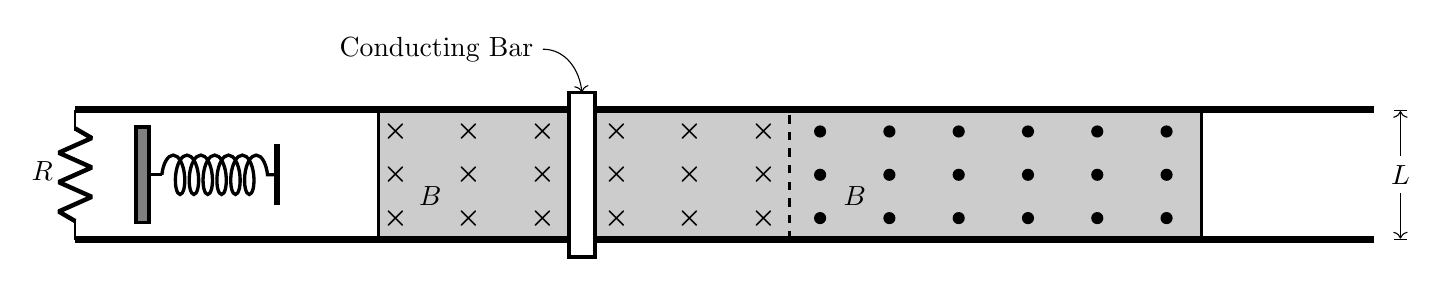
\begin{tikzpicture}[scale=1.1]%[circuit ee IEC]
      \draw[very thick,fill=lightgray!80] (3.5,0) rectangle (13,1.5);
      \draw[very thick,dashed] (8.25,0)--+(0,1.5);
      \foreach \y in {0,1.5} \draw[line width=2.5] (0,\y)--+(15,0);
      \draw[thick,
        every resistor/.style={circuit symbol size=tiny}
        ] (0,0) to[resistor,l=$R$] (0,1.5);
      \draw[|<->|] (15.3,0)--+(0,1.5) node[midway,fill=white]{$L$};
      \draw[very thick,fill=white] (5.7,-.2) rectangle +(.3,1.9);
      \draw[<-] (5.85,1.7) to[out=95,in=0] (5.4,2.2) node[left]{Conducting Bar};
      
      \foreach \x in {8.6,9.4,...,13}{
        \foreach \y in {.25,.75,1.25} \fill (\x,\y) circle (.07);
      }
      \foreach \x in {3.7,4.55,...,8.3}{
        \foreach \y in {.25,.75,1.25} \node at (\x,\y) {$\bm\times$};
      }
      \draw[very thick,fill=gray] (.7,.2) rectangle +(.15,1.1);
      \fill (2.3,.4) rectangle +(.07,.7);
      \draw[very thick,
        decoration={aspect=.4,segment length=5, amplitude=2.5mm, coil},
        decorate] (1,.75)--(2.3,.75);
      \draw[very thick] (.85,.75)--(1,.75);

      \node at (4.1,.5) {$B$};
      \node at (9,.5) {$B$};
    \end{tikzpicture}
    
    Top View (at time $t_B$)
  }
  \question Two horizontal, parallel, conducting rails are separated by
  distance $L=\SI{.40}\metre$. A resistor of resistance $R=\SI{.30}\ohm$
  connects the rails. A horizontal ideal spring is located between the rails.
  The right end of the spring is free to move and the left end is fixed in
  place. A conducting bar of mass $m=\SI{.23}{\kilo\gram}$ is placed on the
  rails and is n contact with the spring, which is initially compressed.
  Frictional forces and the resistance of the bar and rails are negligible.
  \begin{itemize}[itemsep=0pt]
  \item At time $t=0$, the bar is released from rest and is pushed to the right
    by the spring.
  \item At time $t_1$, the bar loses contact with the spring and slides to the
    right.
  \item At time $t_2$, the bar enters and travels through a uniform magnetic
    field of magnitude $B=\SI{.50}\tesla$ that is directed into the page, as
    shown.
  \item At time $t_3$, the bar enters a region where the magnitude of the
    uniform magnetic field is still $B=\SI{.50}\tesla$ but is directed out of
    the page.
  \item At time $t_4$, the bar enters a region with no magnetic field.
  \end{itemize}

  Consider time $t_B$ such that $t_2<t_B<t_3$.
  \begin{parts}
  \item On the following diagram of the bar, draw an arrow indicating the
    direction of the net force $F_\text{net}$ exerted on the bar at time $t_B$.
    If the net force is zero, write $F_\text{net}=0$.
    \begin{center}
      \vspace{.3in}
      {\tikz\draw[thick] rectangle (.3,1.9);}
    \end{center}
    \newpage

    \uplevel{
      At time $t_B$, the speed of the bar is $v=\SI{2.5}{\metre\per\second}$.
    }
    \part Calculate the magnitude of the current in the bar at time $t_B$.
    \vspace{\stretch1}

    \part Calculate the magnitude of the net force $F_\text{net}$ exerted on the
    bar at time $t_B$.
    \vspace{\stretch1}

    \part On the following axes, sketch a graph of the speed $v$ of the bar as
    a function of time $t$ between $t=0$ and $t_4$.
    \uplevel{
      \centering
      \begin{tikzpicture}
        \draw[axes] (0,0)--(7,0) node[right]{$t$} node[pos=0,below left]{$O$};
        \draw[axes] (0,0)--(0,4) node[above]{$v$};
        \draw[dashed] (1.7,0)--+(0,3.7) node[pos=0,below]{$t_1$};
        \draw[dashed] (3,0)--+(0,3.7) node[pos=0,below]{$t_2$};
        \draw[dashed] (4.7,0)--+(0,3.7) node[pos=0,below]{$t_3$};
        \draw[dashed] (6.5,0)--+(0,3.7) node[pos=0,below]{$t_4$};
      \end{tikzpicture}
    }
    \newpage

    \uplevel{
      \begin{center}
        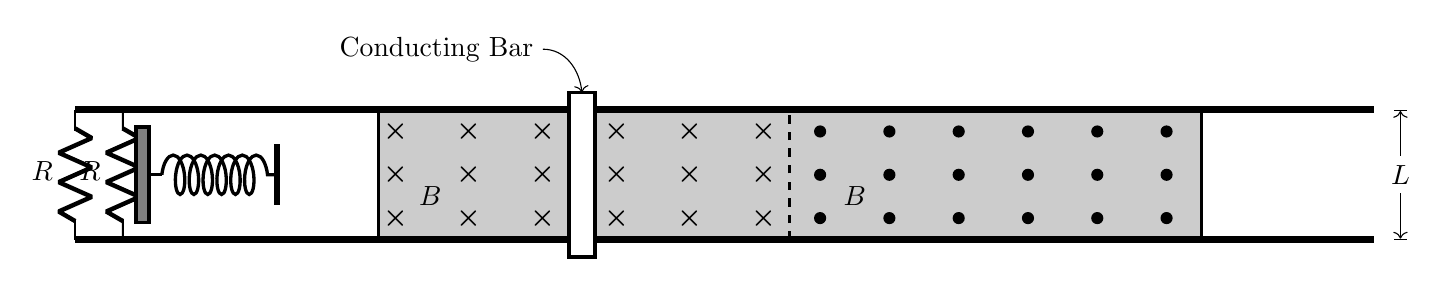
\begin{tikzpicture}[scale=1.1]%[circuit ee IEC]
          \draw[very thick,fill=lightgray!80] (3.5,0) rectangle (13,1.5);
          \draw[very thick,dashed] (8.25,0)--+(0,1.5);
          \foreach \y in {0,1.5} \draw[line width=2.5] (0,\y)--+(15,0);
          \draw[thick] (0,0) to[resistor,l=$R$] +(0,1.5);
          \draw[thick] (.55,0) to[resistor,l=$R$] +(0,1.5);
          \draw[|<->|] (15.3,0)--+(0,1.5) node[midway,fill=white]{$L$};
          \draw[very thick,fill=white] (5.7,-.2) rectangle +(.3,1.9);
          \draw[<-] (5.85,1.7) to[out=95,in=0] (5.4,2.2)
          node[left]{Conducting Bar};
      
          \foreach \x in {8.6,9.4,...,13}{
            \foreach \y in {.25,.75,1.25} \fill (\x,\y) circle (.07);
          }
          \foreach \x in {3.7,4.55,...,8.3}{
            \foreach \y in {.25,.75,1.25} \node at (\x,\y) {$\bm\times$};
          }
          \draw[very thick,fill=gray] (.7,.2) rectangle +(.15,1.1);
          \fill (2.3,.4) rectangle +(.07,.7);
          \draw[very thick,
            decoration={aspect=.4,segment length=5, amplitude=2.5mm, coil},
            decorate] (1,.75)--(2.3,.75);
          \draw[very thick] (.85,.75)--(1,.75);

          \node at (4.1,.5) {$B$};
          \node at (9,.5) {$B$};
        \end{tikzpicture}
    
        Top View (at time $t_B$)
      \end{center}
      
      The scenario is repeated but an additional resistor of resistance
      $R=\SI{.30}\ohm$ is connected, as shown.
    }

    \part Determine the total resistance $R_\text{total}$ of the closed circuit
    for the new scenario.
    \vspace{\stretch1}
    
    \part In the original scenario, the magnitude of the acceleration of the
    bar immediately after the bar enters the first uniform magnetic field is
    $a_\text{original}$. In the new scenario, the magnitude of the acceleration
    of the bar immediately after the bar enters the first uniform magnetic
    field is $a_\text{new}$. Is a new greater than, less than, or equal to
    $a_\text{original}$? \textbf{Justify} your answer.
    \vspace{\stretch1}
    
    \part\textbf{Describe} a modification to $m$, $B$, or $L$ that will result
    in a smaller induced potential difference across the original resistor
    immediately after the bar enters the first uniform magnetic field.
    \textbf{Justify} your answer.
    \vspace{\stretch1}
  \end{parts}
\end{questions}
\end{document}
